% ju 11-Aug-20
\documentclass[a4paper,12pt]{scrartcl}
% letztes Update: 1-Jun-20

% Eingabe der Metadaten

%-------Daten des Autors--------------------------
\newcommand{\autor}{Jan Unger}
\newcommand{\ort}{Wuppertal}
\newcommand{\website}{https://bw-ju.de/}

%-------Titel und Untertitel-----------------------
\newcommand{\titel}{Vektorgrafiken in SVG und EPS}% THEMA 
\newcommand{\untertitel}{\LaTeX -- WEB}% keinen Untertitel 
\newcommand{\typ}{Projekt}

%-------Datum: Jahr/Monat/Tag ---------------------
\newcommand{\version}{\today}% DATUM:  \date{2020/06/30}  o. \today

%-deutsche Schlagwoerter(bitte getrennt durch Kommata auflisten)
\newcommand{\schlagwoerter}{PDF, Latex, Markdown, Pandoc, Git, Texlive}



%% anpassen
\usepackage{praeambel-artikel}% Pakete
% Literatur laden
\bibliography{content/literatur}      %% anpassen
\bibliography{content/literatur-kfz}  %% anpassen
\bibliography{content/literatur-sport}%% anpassen
%% anpassen
\title{Spickzettel-LaTeX}
\author{\autor}
\date{\today}
%\date{2020/08/01}%% anpassen
%\date{1-Aug-20}
%
\begin{document}
	%% anpassen
	%\maketitle
	%\tableofcontents  
	%\listoffigures 
	%\listoftables 
	%\lstlistoflistings

	%% anpassen	
	%\begin{abstract}
	%	Zusammenfassung
	%\end{abstract}

	%% anpassen
	%-------------------------------------------------
	%
		% letztes Update: 20-Okt-19
%\chapter{Spickzettel -- \LaTeX}

\section{Quellenangabe}\label{sec:quellenangabe}\index{Quellenangabe}

\verb|\textcite|

Zitat: vgl. \textcite{monk:2016:action} und \textcite{kofler:2017:linux}.

Quelle: \textcite{kofler:2018:hacking}.

Quelle: \textcite[87]{schmidt:2015:klima} und \textcite{schneehage:2018:aktoren}.

vgl. \textcite{zeller:2017:hindernis}, \textcite{marquardt:2018:trainingsplan10km} und \textcite{lauren:2017:fit}.


\section{Referenz und Links}\label{sec:referenzlinks}\index{Referenz}

\begin{itemize}
	\item Link \footnote{\url{https://bw-ju.de/}} \verb|\footnote{\url{}}|
	\item Link \url{https://bw-ju.de/} \verb|\url{}|
	\item Link auf File \url{https://github.com/ju1-eu/dummy-notizenUbuntu-v03/blob/master/README.pdf}
	\item Referenz auf Bild (\autoref{fig:bild}). \verb|(\autoref{fig:}).|
	\item Referenz auf Tabellen (\autoref{tab:tabellen}). \verb|(\autoref{tab:}).|
	\item Referenz auf Kapitel (\autoref{sec:zusammenfassung}). \verb|(\autoref{sec:}).|
 	\item Referenz auf Code (\autoref{code:halloweltex}). \verb|(\autoref{code:}).|
	\item Textfußnote \footnote{Fußnote} \verb|\footnote{}|
\end{itemize}


\section{Quellcode}\index{Quellcode}

Programmiersprache C++ (\autoref{code:halloweltex}).
\lstset{language=C++}% C, TeX, Bash, Python
\lstinputlisting[%% anpassen
caption={Programmiersprache C++},label={code:halloweltex}]
{content/beispiele/code/hallo-c++.cpp}


\LaTeX -Syntax (\autoref{code:latexsyntax}). 
\lstset{language=TeX}% C, TeX, Bash, Python
\begin{lstlisting}[%% anpassen
caption={\LaTeX-Syntax},label={code:latexsyntax}]
% artikel.tex
\documentclass[a4paper, 12pt, fleqn, parskip=half]{scrartcl}
\usepackage[ngerman]{babel}
\usepackage[utf8]{inputenc}
\usepackage{times}
\usepackage{booktabs}
\usepackage{graphicx}
\begin{document}
Hallo Welt!
\end{document}
\end{lstlisting}

\section{Text und Absatz}\index{Absatz}

Dies ist ein Typoblindtext für die Anleitung. Dies ist ein Typoblindtext für die Anleitung.
Dies ist ein Typoblindtext für die Anleitung.

\noindent Dies ist ein Typoblindtext für die Anleitung.

\noindent Dies ist ein Typoblindtext für die Anleitung. Dies ist ein Typoblindtext für die Anleitung.
Dies ist ein Typoblindtext für die Anleitung. 
\vspace{1cm}

\noindent Dies ist ein Typoblindtext für die Anleitung.

\section{Index}

Dies ist ein kurzer \index{kurz} Satz.

\noindent Die ist ein neuer \index{neu} Satz.

\section{Bilder}\label{sec:bild}

Bild (\autoref{fig:bild}).
\begin{figure}[!h]% hier: !hb
	\centering
	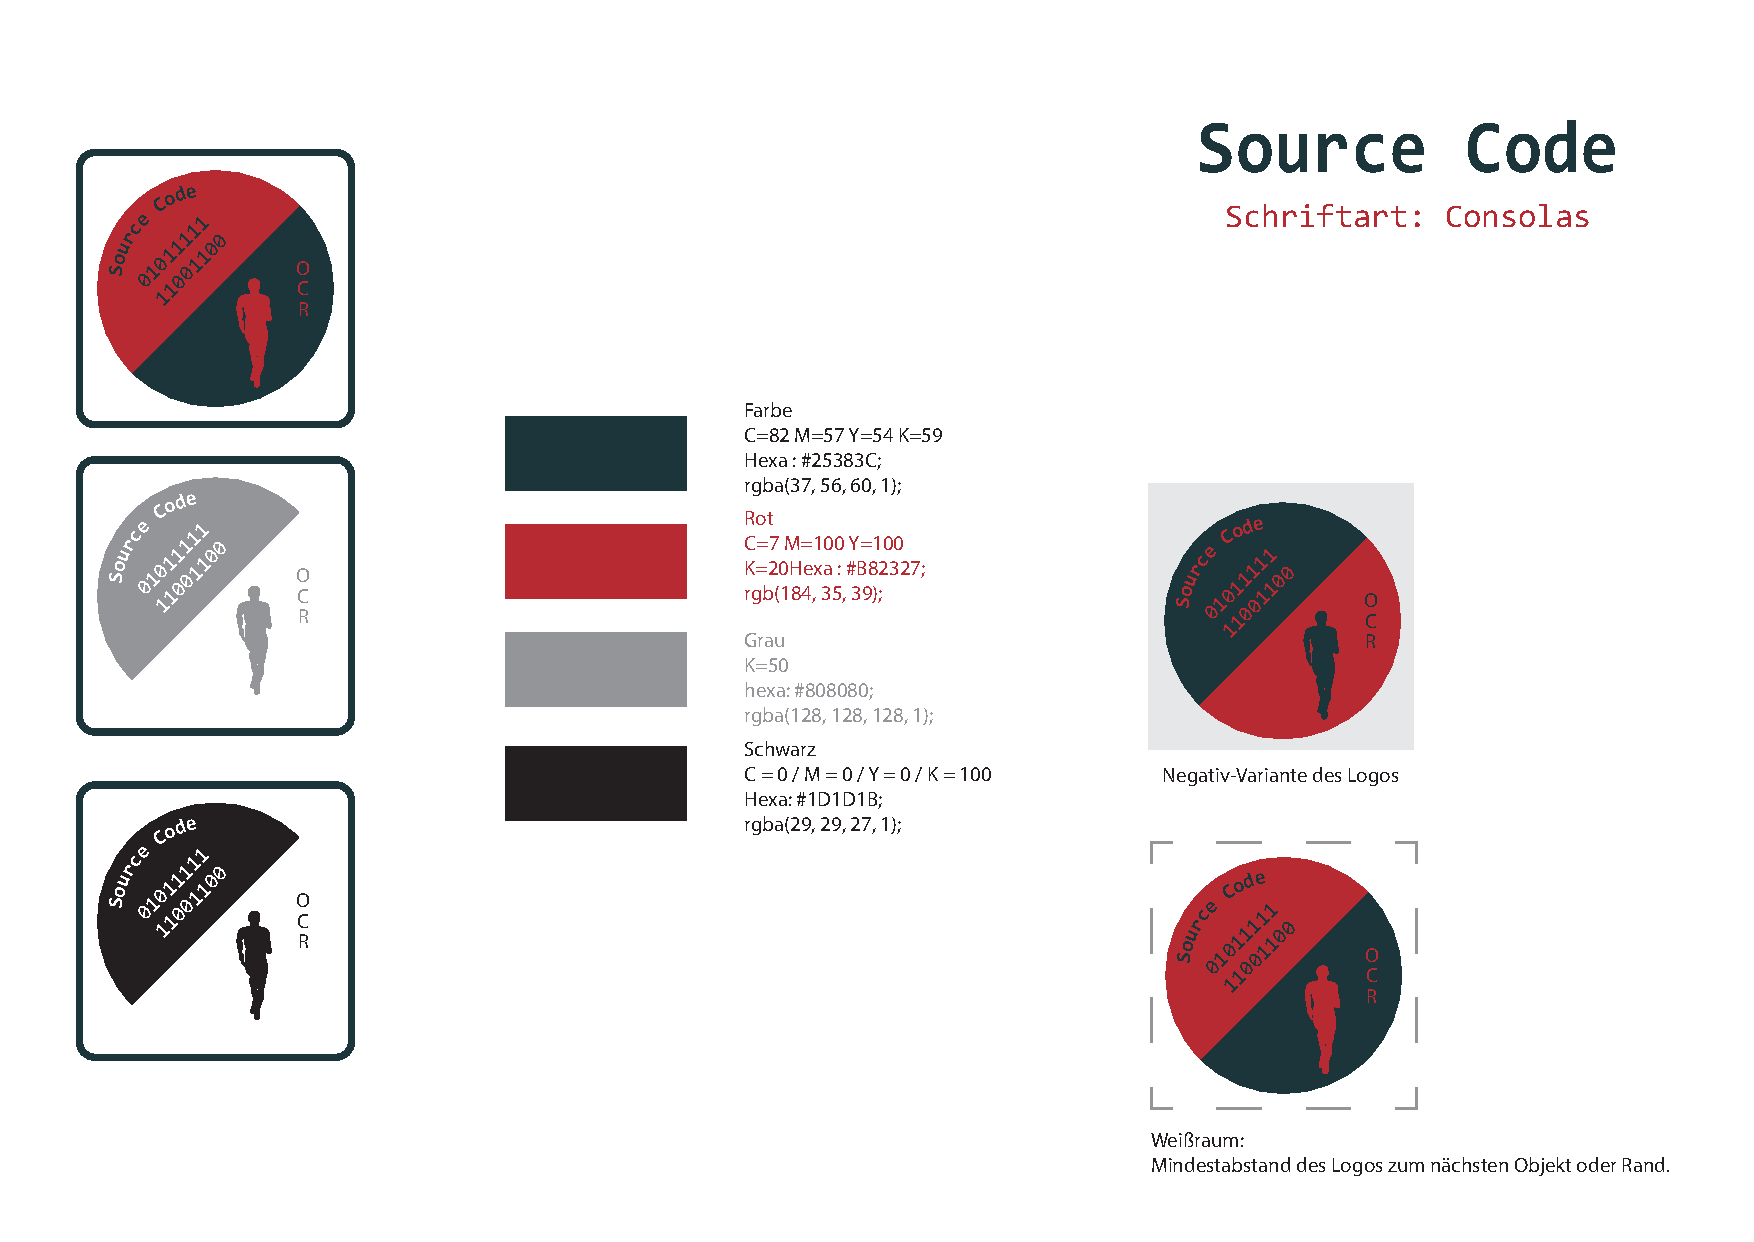
\includegraphics[width=.55\textwidth]{content/beispiele/images/Logo-Details.eps}
	\caption{Bild}\label{fig:bild}%% anpassen
\end{figure}


Logo in Negativ, Grau u. Schwarz (\autoref{fig:logonegativgrauschwarz}).
\begin{figure}[!h]% hier: !hb
	\centering
	\begin{minipage}[b]{0.40\textwidth}
		
\includegraphics[width=\textwidth]{content/beispiele/images/Logo-negativ.eps}
	\end{minipage}
	\hfill
	\begin{minipage}[b]{0.30\textwidth}
		
\includegraphics[width=\textwidth]{content/beispiele/images/Logo-Grau.eps}
	\end{minipage}
	\hfill
	\begin{minipage}[b]{0.20\textwidth}
		
\includegraphics[width=\textwidth]{content/beispiele/images/Logo-SW.eps}
	\end{minipage}
	\caption{Logo in Negativ, Grau u. Schwarz
	  \newline Quelle: https://bw-ju.de/}\label{fig:logonegativgrauschwarz}%% anpassen
\end{figure}

Logo Details (\autoref{fig:logodetails}).
\begin{figure}[!h]% hier: !hb
	\centering
	\begin{minipage}[b]{0.49\textwidth}
		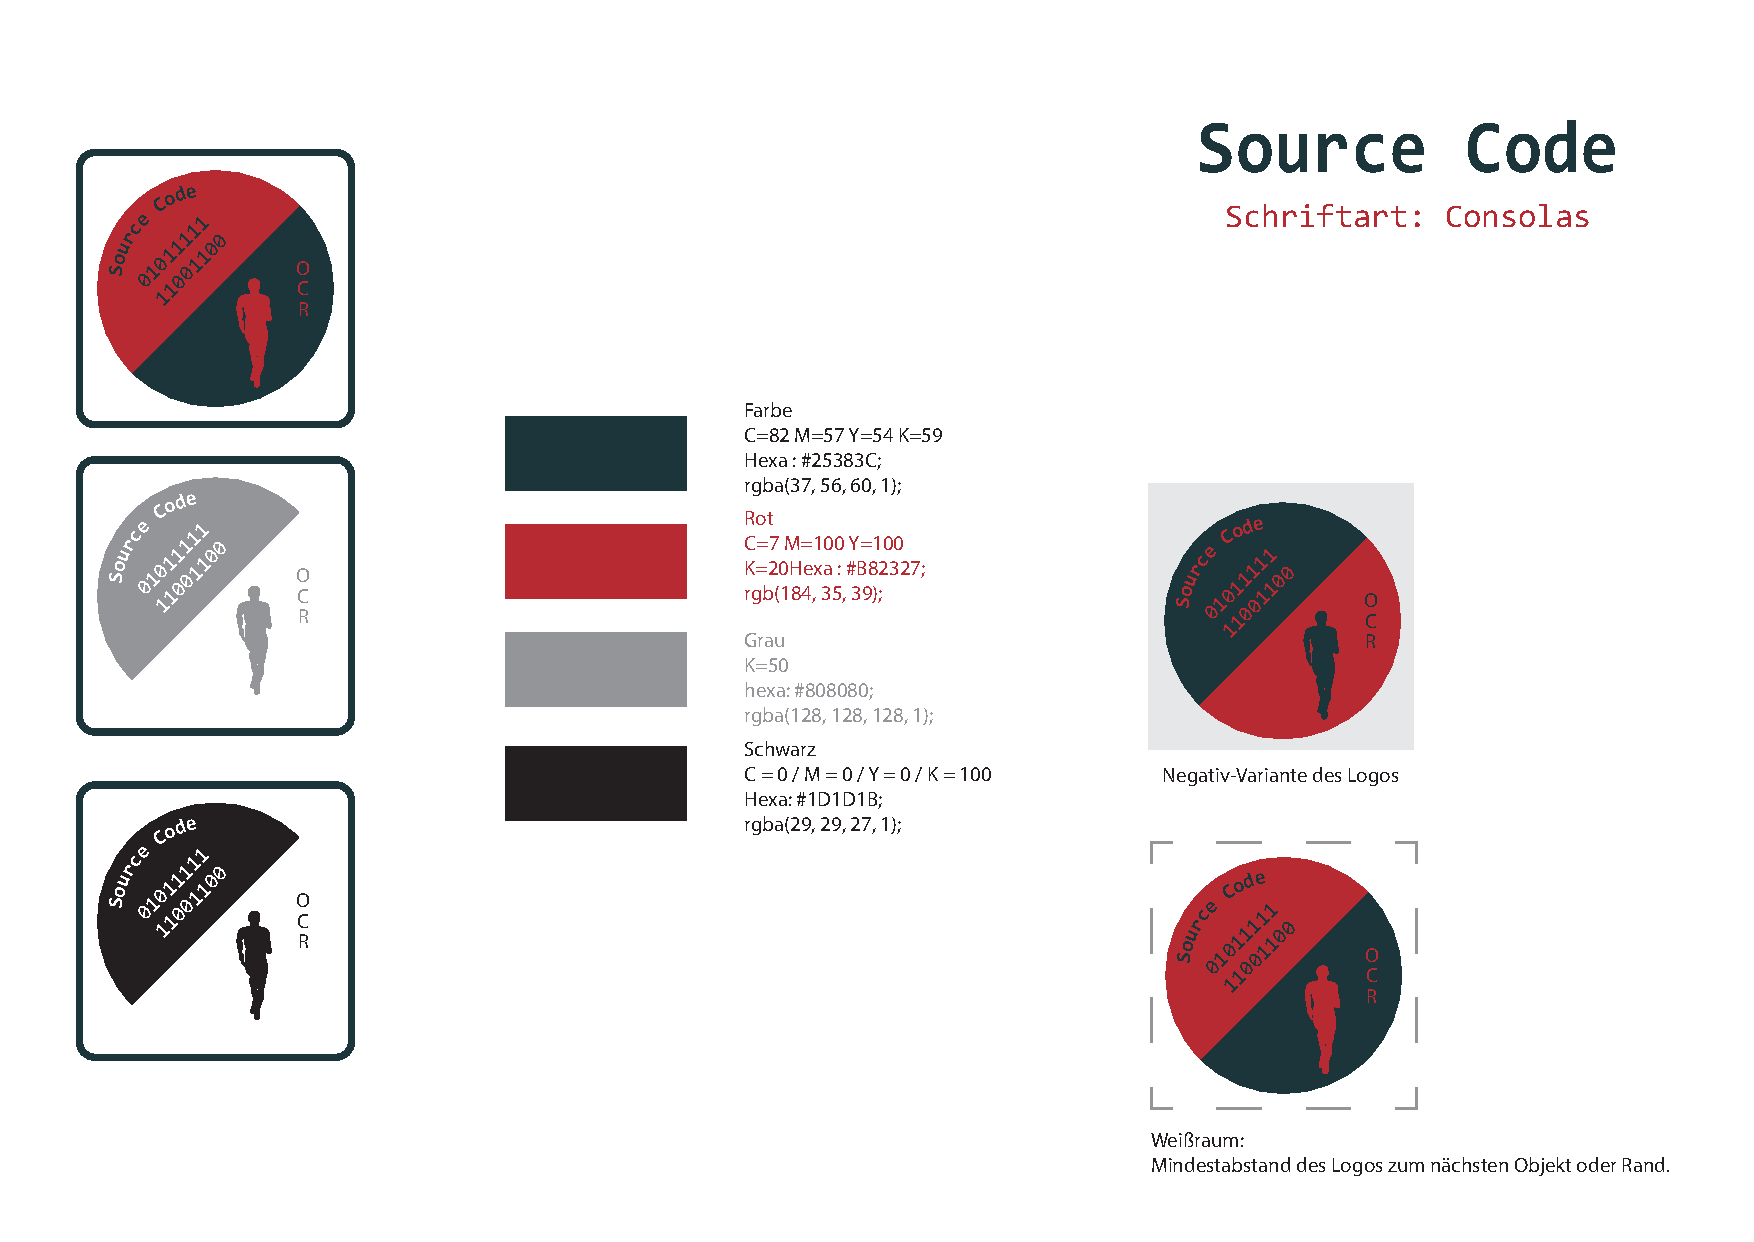
\includegraphics[width=\textwidth]{content/beispiele/images/Logo-Details.eps}
	\end{minipage}
	\hfill
	\begin{minipage}[b]{0.49\textwidth}
		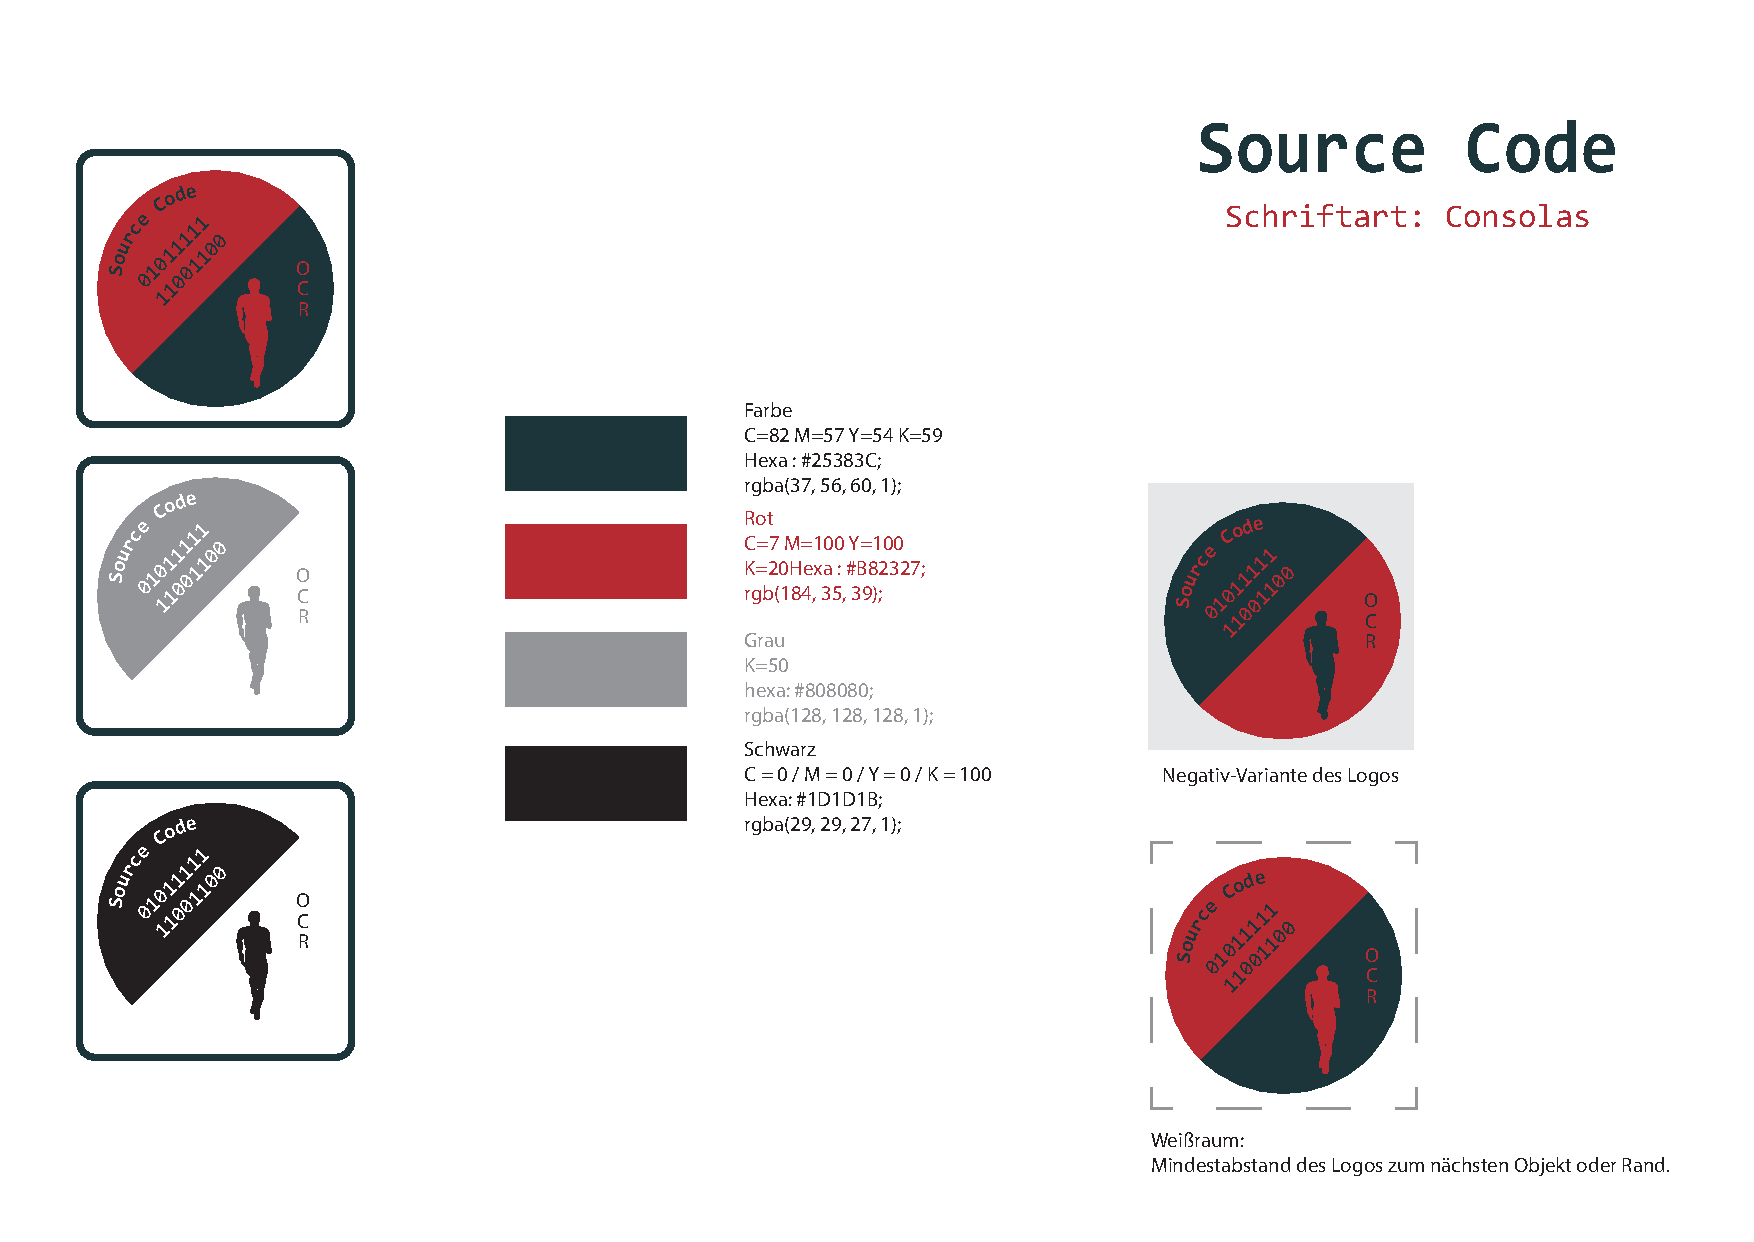
\includegraphics[width=\textwidth]{content/beispiele/images/Logo-Details.eps}
	\end{minipage}
	\caption{Logo Details}\label{fig:logodetails}%% anpassen
\end{figure}

\section{Tabellen}
\label{sec:tabellen}

 Tabelle (\autoref{tab:tabellen}). 
\begin{table}[!h]% hier: !ht
	\centering 
    \caption{Tabellen}\label{tab:tabellen}%% anpassen
	\begin{tabular}{@{}rlc@{}}
	\toprule 
    \textbf{Nr.} & \textbf{Begriffe} & \textbf{Erklärung}\\
	\midrule
    1 & a1 & a2\\
    2 & b1 & b2\\
    3 & c1 & c2\\
    4 & a1 & a2\\
	\bottomrule
 	\end{tabular}
\end{table}


\noindent
%\centering
\begin{tabular}[2]{|p{3cm}|p{9cm}|}
	\hline
	\textbf{Teil} & \textbf{Beschreibung} \\ \hline
	Batterie & Versorgt das System mit Strom. Hat einen ungeregelten Spannungsbereich von ca. 11,5 V - 16,75 V je nach Ladezustand \\ \hline
	Schalter & mechanische Trennung der elektrischen Energie zum Rest des Roboters \\ \hline
\end{tabular}
\bigskip

\noindent
%\centering
\begin{tabular}[3] {| l | l | l |}
	\hline
	\textbf{Control Board Label} & \textbf{Wire Color} & \textbf{Signal} \\ \hline
	VCC & Red & Motor + \\ \hline
	GND & Black & GND \\ \hline
\end{tabular} 


\section{Matheumgebung}\label{sec:matheumgebung}

\begin{equation}\label{eq:mass}%% anpassen
	d_1 = 7.254~mm \qquad d_2 = d_3 = 10.5~mm \qquad d_4 = 10.073~mm
\end{equation}

\begin{equation}\label{eq:kleiner}%% anpassen
	1 \le 2 \ge 0 \neq 4, \quad 1 \ll 10^{20} \gg 10^{-5} \pm 
\end{equation}

\begin{equation}\label{eq:produkt}%% anpassen
	a \cdot b \quad
	a \times b \quad
	\frac x2 \quad
	a_1 \quad
	a^2 \quad
	\binom{a}{b} \quad
	\sqrt{x} \quad bzw. \quad \sqrt[n]{x} \quad	
\end{equation}

\begin{equation}\label{eq:summe2}%% anpassen
	\sum \limits_{i=1}^n i = \frac{n(n+1)}{2}
\end{equation}

\begin{equation}\label{eq:fak}%% anpassen
	\prod \limits_{i=1}^{n+1}i = 1\cdot 2\cdot\dots\cdot n\cdot (n+1)
\end{equation}

\begin{equation}\label{eq:lim}n
	\lim\limits_{n \to \infty}\frac{1}{n}=0
\end{equation}

\begin{equation}\label{eq:matrix}%% anpassen
	\left(
	\begin{array}{ccc}
		a_{11} & \cdots & a_{1n} \\
		\vdots & \ddots & \vdots \\
		a_{m1} & \cdots & a_{mn}
	\end{array}
	\right)	
\end{equation}


\section{Farben}\label{sec:farben}

\begin{itemize}
	%\textcolor{}{} \colorbox{}{}
	\item[] \colorbox{Apricot}{Apricot} \textcolor{Apricot}{Apricot}
	\item[] \colorbox{Cyan}{Cyan}  \colorbox{Mahogany}{Mahogany} 	\colorbox{SpringGreen}{SpringGreen}
	\item[] \colorbox{Aquamarine}{Aquamarine}	\colorbox{Dandelion}{Dandelion}	\colorbox{Maroon}{Maroon}	\colorbox{Purple}{Purple}	\colorbox{Tan}{Tan}
	\item[] \colorbox{DarkOrchid}{DarkOrchid}	\colorbox{Melon}{Melon}	\colorbox{RawSienna}{RawSienna}		\colorbox{TealBlue}{TealBlue}
	\item[] \colorbox{Black}{Black}	 \colorbox{Emerald}{Emerald}		\colorbox{MidnightBlue}{MidnightBlue}     \colorbox{Red}{Red}	\colorbox{Thistle}{Thistle}
	\item[] \colorbox{Blue}{Blue}	   \colorbox{ForestGreen}{ForestGreen}	\colorbox{Mulberry}{Mulberry}		\colorbox{RedOrange}{RedOrange}		\colorbox{Turquoise}{Turquoise}
	\item[] \colorbox{BlueGreen}{BlueGreen}	\colorbox{Fuchsia}{Fuchsia}		\colorbox{NavyBlue}{NavyBlue}	 \colorbox{RedViolet}{RedViolet}		\colorbox{Violet}{Violet}
	\item[] \colorbox{BlueViolet}{BlueViolet}	\colorbox{Goldenrod}{Goldenrod}	\colorbox{OliveGreen}{OliveGreen}		\colorbox{Rhodamine}{Rhodamine}	  	\colorbox{VioletRed}{VioletRed}
	\item[] \colorbox{Gray}{Gray}	\colorbox{Orange}{Orange}	\colorbox{RoyalBlue}{RoyalBlue}	\colorbox{White}{White}
	\item[] \colorbox{Brown}{Brown}	\colorbox{Green}{Green}		\colorbox{OrangeRed}{OrangeRed}		\colorbox{RoyalPurple}{RoyalPurple}		\colorbox{WildStrawberry}{WildStrawberry}
	\item[] \colorbox{BurntOrange}{BurntOrange}	\colorbox{GreenYellow}{GreenYellow}	\colorbox{Orchid}{Orchid}	 \colorbox{RubineRed}{RubineRed}		\colorbox{Yellow}{Yellow}
	\item[] \colorbox{CadetBlue}{CadetBlue}	\colorbox{JungleGreen}{JungleGreen}	\colorbox{Peach}{Peach}		\colorbox{Salmon}{Salmon}	\colorbox{YellowGreen}{YellowGreen}
	\item[] \colorbox{CarnationPink}{CarnationPink}	\colorbox{Lavender}{Lavender} \colorbox{Periwinkle}{Periwinkle}	\colorbox{SeaGreen}{SeaGreen}         \colorbox{YellowOrange}{YellowOrange}
	\item[] \colorbox{Cerulean}{Cerulean}	\colorbox{LimeGreen}{LimeGreen}	\colorbox{PineGreen}{PineGreen}	\colorbox{Sepia}{Sepia}
	\item[] \colorbox{CornflowerBlue}{CornflowerBlue}	\colorbox{Magenta}{Magenta}	\colorbox{Plum}{Plum}	 \colorbox{SkyBlue}{SkyBlue}
\end{itemize} 


\section{Zusammenfassung}\label{sec:zusammenfassung}

\mybox{
	Es gibt ein paar wichtige Dinge, die beachtet werden sollten, 
    wie bei jedem Projekt, bei dem mit Batterie oder elektrischem Strom gearbeitet wird:

	\noindent \textbf{DIE BATTERIE}. 
}

	%
	%-------------------------------------------------

	%\printindex% Index (Register)
	% Bibliographie
	%\phantomsection\addcontentsline{toc}{section}{Literatur}
	\printbibliography% Literaturverzeichnis
\end{document}
